\documentclass[11pt]{article}

% Basic setup
\usepackage{cmap}
\usepackage[utf8]{inputenc}
\usepackage[T2A]{fontenc}
\usepackage[english]{babel}

% Sans serif font by default
\renewcommand\familydefault{\sfdefault}

% Document margins
\usepackage[margin=2.5cm]{geometry}

% \includegraphics, used to include a picture of me
\usepackage{graphicx}

% === Typography ===

% == Boxes ==
\usepackage{adjustbox}
\usepackage{calc}
\usepackage{tabularx}

% == Colors ==
\usepackage[usenames,dvipsnames]{color}
\definecolor{CvRuleColor}{gray}{0.5}
\definecolor{CvWorkplaceHeaderColor}{gray}{0.97}

% == URLs ==
\usepackage[colorlinks=true,urlcolor=blue]{hyperref}

% == Paragraphs ==
\usepackage{parskip}
\setlength\parindent{0cm}
\setlength\parskip{0cm}

% == Lists ==
\usepackage{enumitem} % [noitemsep]

% === Custom commands ===

% "C++", thanks to this guy: http://tex.stackexchange.com/a/4304/9088
\usepackage{relsize}
\newcommand\CXX{C\nolinebreak[4]\hspace{-.05em}\raisebox{.4ex}{\relsize{-3}{\textbf{++}}}}

% Whitespace
\newcommand\CvSmallSkipLength{0.5em}
\newcommand\CvBigSkipLength{1em}

\newcommand\CvSkip[1]{\vspace{#1}}

\newcommand\CvSmallSkip{\CvSkip{\CvSmallSkipLength}}
\newcommand\CvBigSkip{\CvSkip{\CvBigSkipLength}}

% Section headers ("Experience", "Education", etc.)
\newcommand\CvSectionHeader[1]{\CvBigSkip\textbf{#1}\CvBigSkip}

% Horizontal line/separator
\newcommand\CvRule{\begingroup\color{CvRuleColor}\hrule\endgroup}

% Workplace header
\newcommand\CvWorkplaceHeader[5]{\begingroup%
  \CvRule%
  \fboxsep0pt%
  \colorbox{CvWorkplaceHeaderColor}{%
    \begin{minipage}{\linewidth-2\fboxsep}%
\CvSmallSkip%
#1 -- #2 \hfill \textit{#3} at #4 (\href{http://#5/}{#5})%
\CvSmallSkip%
    \end{minipage}%
  }%
  \CvRule%
\endgroup%
}

% Workplace description
\newenvironment{CvWorkplaceDescription}{%
    \begingroup\setlength\parskip{\CvSmallSkipLength}%
  }{%
    \CvSmallSkip\endgroup%
  }

\pagestyle{empty}

\begin{document}

\adjustbox{valign=t}{%
  \begin{minipage}{3.5cm}%
    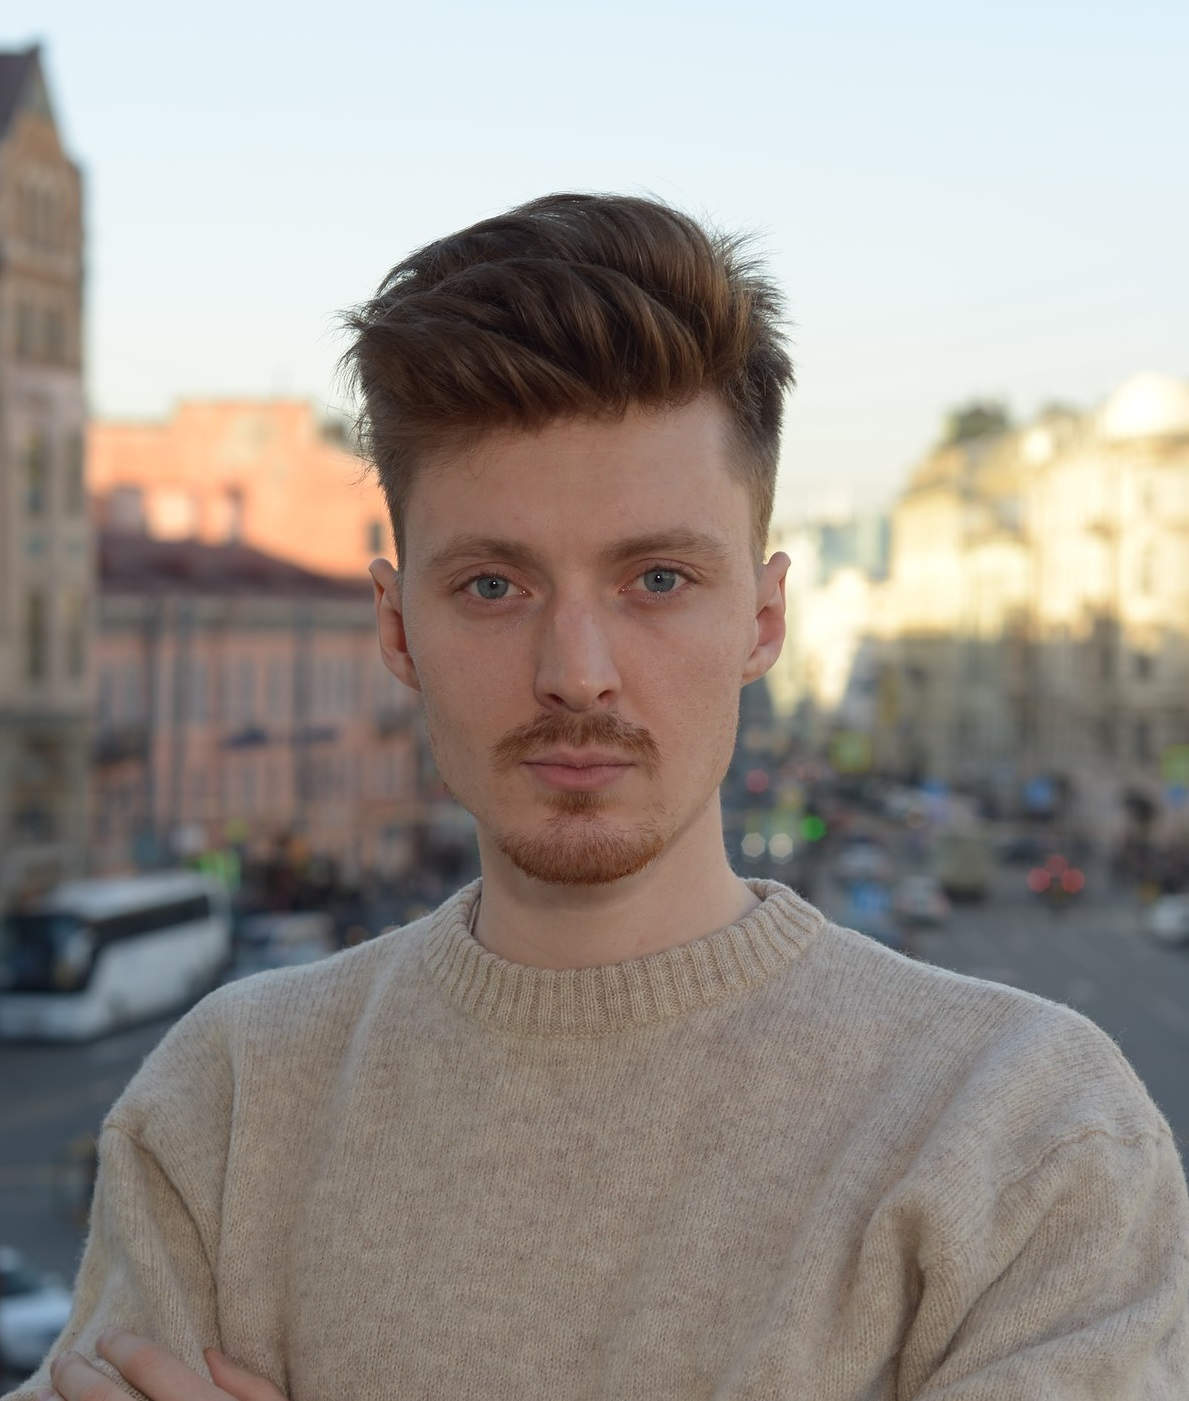
\includegraphics[width=3.5cm]{img/selfie.jpg}
  \end{minipage}%
}%
\hfill%
\adjustbox{valign=t}{%
  \begin{minipage}{\linewidth-3.5cm-\CvBigSkipLength}%
{\bfseries\large Alexey Polusov}\\*
{\color{CvRuleColor} Last updated on: \today}
    \CvBigSkip
    \CvRule
    \CvSmallSkip
    \begin{tabularx}{\textwidth}{@{}lX}
email: & \href{mailto:lectricas@gmail.com}{lectricas@gmail.com} \\
github: & \href{https://github.com/lectricas/}{https://github.com/lectricas/} \\
tel.: & +7\,(952)\,377-09-69 \\
Address: & 1 Tatarskiy Pereulok, apt. 7 \\
& Saint Petersburg, Russia, 197198 \\
    \end{tabularx}%
    \CvSmallSkip
    \CvRule
  \end{minipage}%
}

\CvSectionHeader{Experience}

\CvWorkplaceHeader{October 2018}{Current time}{Lead Android developer}{Firstline Software}{firstlinesoftware.com}
\begin{CvWorkplaceDescription}
First project	 was a mid-size app, then I've took a leading position in a distributed team.
\begin{itemize}[noitemsep]
 \item App for tracking your sugar level
\begin{itemize}
\item  app's key feature is a custom view consist of a infinite graph with scaling and Bezier curve. 
 \item main components of a customView were a: Scroller, GestureDetector(switched to manual onTouch handling), logic was adopted from LinearLayoutManager
\end{itemize}
\item Russian postal service app
\begin{itemize}
\item  This project started a long time ago, and contains a lot of legacy code
\item  App consists of many different features, including payments, GeoFences, Launcher Widgets, AccountManager, Maps, etc.
 \item My job was to coordinate 5 members Android team and implement features
\end{itemize}
\end{itemize}

Key skills \& technologies employed:
\begin{itemize}[noitemsep]
  \item Kotlin, Koin, RxPM, Moxy, Room, RxBindings, RxJava, Retrofit
\end{itemize}
\end{CvWorkplaceDescription}

\CvWorkplaceHeader{September 2017}{October 2018}{Android developer}{MobileUp}{mobileup.ru}

\begin{CvWorkplaceDescription}
I have been taking part in development of several projects, from mid-scale to large ones:
\begin{itemize}[noitemsep]
  \item participated in developing a blockchain-oriented application(+ etherium currency involved),
  \item responsible for all UI logic, I've worked with compound views and animations
  \item get acquainted with blockchain development
  \item fixed a few other projects adding some new features,
  \item configured Bitbucket CI was trying others: Jenkins, AppCenter(we lack some devices), TeamCity,
\end{itemize}

Key skills \& technologies employed:
\begin{itemize}[noitemsep]
  \item Kotlin for sure!,
  \item RxPm(MVVM like library baked in MobileUp),
  \item RxJava, Dagger2, Koin, RxBinding, Conductor, web3j for blockchain
  \item Room, Architecture Components, BiometricPrompt, etc
\end{itemize}
\end{CvWorkplaceDescription}

\CvWorkplaceHeader{February 2016}{August 2017}{Android developer}{65apps}{www.65apps.com}

\begin{CvWorkplaceDescription}
I have been taking part in development of a mid-scale projects as a member of an Android team. I was responsible for developing different app features and support components:
\begin{itemize}[noitemsep]
  \item done one middle-size news project from scratch(GP published and successful),
  \item developed multiply features for several projects,
  \item bug fixes for projects on "support",
\end{itemize}

Key skills \& technologies employed:
\begin{itemize}[noitemsep]
  \item Java programming in Android Studio,
  \item CLEAN architecture supported by Dagger 2 and Moxy,
  \item RxJava, Retrofit, Firebase, Butterknife, etc
  \item GitFlow
\end{itemize}
\end{CvWorkplaceDescription}

\CvRule

\CvSectionHeader{Education}

\CvWorkplaceHeader{2009}{2013}{Bachelor of Information Security}{ISTU}{http://istu.ru/}

\begin{CvWorkplaceDescription}
During my education, I've been focusing on the following topics:
\begin{itemize}[noitemsep]
  \item hidden electronic devices for listen in,
  \item hardware key interceptor, masked as a USB - PS/2 adapter
\end{itemize}
\end{CvWorkplaceDescription}
\CvRule

\begin{minipage}[t]{.5\linewidth}
  \CvSectionHeader{Programming Languages}

  \begin{itemize}
    \item Java, Kotlin, Python
  \end{itemize}

  \CvSectionHeader{Development Tools \& Technologies}

  \begin{itemize}
    \item Bitbucket CI, AppCenter, TeamCity
    \item Heroku, PythonAnywhere, Parse
   \item Git
   \item Bash
   \item some SQL
  \end{itemize}

  \CvSectionHeader{Hobbies}

  \begin{itemize}
    \item Sometimes I code to learn new things. 
 \item Interested in graphics and sound in Android system.
   \item road bike riding, jogging
  \end{itemize}
\end{minipage}
\begin{minipage}[t]{.5\linewidth}
  \CvSectionHeader{Languages}

  \begin{itemize}
    \item Russian --- mother tongue.
    \item English --- TOEFL 93 score a few years ago(trying to sustain the level).
  \end{itemize}

  \CvSectionHeader{Other Tools \& Technologies}

  \begin{itemize}
    \item postman
   \item Word, Excel, Photoshop
    \item Thinkpad lover, Google Pixel fan
    \item \LaTeX
  \end{itemize}
\end{minipage}

\end{document}